% ============================================================
%  IEEE Transactions on Power Delivery
%  "Coordinated Adaptive Overcurrent Protection for Parallel
%   Synchronous Generators Using Online Inverse Estimation"
%  Author: J. Eluvathingal
%  Build:  pdflatex × 3 + bibtex
% ============================================================
\documentclass[journal,twoside,letterpaper]{IEEEtran}

%% --- packages ---------------------------------------------------
\usepackage[T1]{fontenc}
\usepackage[utf8]{inputenc}
\usepackage{amsmath,amssymb,bm}
\usepackage{graphicx}
\usepackage{xcolor}
\usepackage{booktabs}
\usepackage{multirow}
\usepackage{cite}
\usepackage{url}
\usepackage{siunitx}
\usepackage{gensymb}
\usepackage{algorithm}
\usepackage{algpseudocode}
\usepackage{tikz}
\usepackage{pgfplots}
\pgfplotsset{compat=1.18}
\usetikzlibrary{positioning,shapes.geometric,shapes.misc,
                arrows.meta,chains,decorations.pathreplacing,
                calc,fit}
\usepgfplotslibrary{groupplots,fillbetween}

%% --- helpers ---------------------------------------------------
\newcommand{\vect}[1]{\bm{#1}}
\newcommand{\est}[1]{\hat{#1}}
\newcommand{\norm}[1]{\lVert#1\rVert}
\DeclareMathOperator{\clip}{clip}
\newtheorem{proposition}{Proposition}

%% --- document --------------------------------------------------
\begin{document}

\title{Coordinated Adaptive Overcurrent Protection for Parallel
       Synchronous Generators Using Online Inverse Estimation}

\author{Anoop~V.~Eluvathingal,~\IEEEmembership{Student Member,~IEEE,}
        and~K.~Shanti~Swarup,~\IEEEmembership{Senior Member,~IEEE}%
\thanks{Manuscript received \today.
        This work is part of the PhD research programme at the Department of
        Electrical Engineering, Indian Institute of Technology Madras,
        Chennai~600~036, India, and extends the SAMBP-SyncOC Stage-1
        framework (SAMBP TR-01/2026) with a supervisory coordination layer.}%
\thanks{A.~V.~Eluvathingal and K.~S.~Swarup are with the Department of
        Electrical Engineering, IIT Madras, Chennai~600~036, India
        (e-mail: ee21d017@smail.iitm.ac.in; swarup@ee.iitm.ac.in).}}

\markboth{IEEE Transactions on Power Delivery,~Vol.~XX,
No.~X, \MakeUppercase{Month}~2026}%
{Eluvathingal \& Swarup: Coordinated Adaptive OC Protection Using Online
Inverse Estimation}

\maketitle

%% =============================================================
\begin{abstract}
Adaptive overcurrent relays driven by online parameter
estimation improve sensitivity on synchronous-generator feeders,
yet their independent per-relay updates can break the
selectivity and time-grading relationships that are the
cornerstone of coordinated protection.
This paper introduces a supervisory coordination layer that
enforces two hard constraints after each local adaptation event:
(i)~pickup selectivity,
$I_{p,k} \geq I_{p,k+1} + \Delta I_m$, and
(ii)~inverse-time grading,
$t_{\mathrm{op},k}(I_{f,\min}) \geq
 t_{\mathrm{op},k+1}(I_{f,\min}) + \Delta t_g$,
across all generator relays referred to a common busbar.
The layer receives the locally estimated fault-current
parameters~$\est{\vect\theta}_k^{(1)}$ from each relay,
computes a coordinated pickup--TMS pair
$\{I_{p,k}^c,\,TMS_k^c\}$
via a greedy cascade and a closed-form TMS correction,
and deploys the results within the same post-fault
adaptation window.
Case studies on a two-generator IEC~60909 study system
demonstrate that without coordination the selectivity
margin collapses from~0.40~p.u.\ (fixed) to~0.157~p.u.\
(local adaptive), violating the required~0.20~p.u.\ margin;
the proposed layer restores the margin to~0.200~p.u.\
while maintaining a time-grading margin of 2.74~s against the
required~0.15~s.
Over a~$4 \times 2$ study matrix (two generators, 3PH and SLG
faults), all scenarios achieve selectivity and grading
compliance with zero false trips.
\end{abstract}

\begin{IEEEkeywords}
adaptive protection, overcurrent relay, coordination,
synchronous generator, inverse estimation, Levenberg--Marquardt,
pickup selectivity, time-grading margin, busbar protection.
\end{IEEEkeywords}

%% =============================================================
\section{Introduction}
\label{sec:intro}

Overcurrent protection of parallel synchronous generators
connected to a common busbar presents a recurring coordination
challenge: the relay on each generator feeder
($R_k$, $k=1,\dots,N$) must operate before the common bus
relay~$R_B$ for faults on the generator side, yet must remain
faster than upstream protection for through-faults
\cite{Anderson1999,Blackburn2006}.
Fixed settings satisfy these requirements at the rated
operating point, but the effective short-circuit level varies
with the number of online generators, the
sub-transient and transient reactances, and the loading
state~\cite{IEEE1110_2002,Kundur1994}.
Consequently, the margins between adjacent relays can
narrow or even invert as the system configuration changes,
compromising either sensitivity or selectivity.

Adaptive overcurrent protection addresses this by adjusting
relay settings in real time.
Early approaches relied on pre-computed setting groups indexed
by a discrete operating mode~\cite{Urdaneta1988,Novosel1994}.
More recently, online estimation methods fit a parametric
fault-current model to the measured waveform, yielding
continuous-valued settings that track the actual source
impedance~\cite{Eluvathingal2025_TR01}.
The Stage-1 inverse estimator of the SAMBP-SyncOC framework
uses a two-pass Levenberg--Marquardt (LM) algorithm to extract
the six-parameter reduced model
$\vect\theta = [t_0,\,I_{ss},\,I_{sub},\,\tau_{ac},\,\tau_{dc},\,\varphi_a]$
and maps the result to adaptive pickup and TMS values via
linear scaling laws~\cite{Eluvathingal2025_TR01}.

A gap exists, however, that has received insufficient attention:
\emph{independent per-relay adaptation is not sufficient when
multiple relays share a common bus}.
Each relay optimises its own settings for the locally observed
fault current; there is no mechanism to preserve the relative
ordering of pickups or the time-grading margin between adjacent
relays.
In a two-generator busbar, the bus relay~$R_B$ may adapt its
pickup upward (because the combined fault current is large)
while the generator relays adapt downward (because their
individual contributions are smaller), narrowing or inverting
the selectivity hierarchy.

This paper makes the following contributions:
\begin{enumerate}
  \item A formal statement of the multi-generator coordination
    problem as a constraint satisfaction problem (CSP) over
    the pickup and TMS settings of all relays on a common
    busbar (Section~\ref{sec:problem}).
  \item A polynomial-time greedy cascade algorithm that
    restores pickup selectivity in a single upstream pass,
    together with a closed-form minimal TMS correction that
    restores time-grading without increasing any relay's
    operating time below the required margin
    (Section~\ref{sec:algorithm}).
  \item A proof that the greedy cascade terminates in at
    most~$N$ iterations and produces settings that satisfy
    both constraints simultaneously
    (Section~\ref{sec:algorithm}, Proposition~1).
  \item Validation on a two-generator IEC~60909 study system
    across 3PH and SLG faults, quantifying selectivity and
    grading margins in all three protection states
    (fixed, local-adaptive, and coordinated)
    (Sections~\ref{sec:system}--\ref{sec:results}).
\end{enumerate}

The remainder of the paper is organised as follows.
Section~\ref{sec:problem} formulates the multi-generator
coordination problem.
Section~\ref{sec:local} reviews the Stage-1 local estimation
layer.
Section~\ref{sec:constraints} defines the coordination
constraints.
Section~\ref{sec:algorithm} presents the enforcement algorithm.
Section~\ref{sec:system} describes the study system.
Section~\ref{sec:results} presents numerical results.
Section~\ref{sec:discussion} discusses practical considerations
and limitations.
Section~\ref{sec:conclusion} concludes.

%% =============================================================
\section{Multi-Generator Protection Problem Formulation}
\label{sec:problem}

\subsection{System topology}

Consider $N$ synchronous generators $G_k$, $k=1,\dots,N$,
each connected via a step-up transformer with leakage
reactance~$X_{Tk}$ to a common busbar.
Each generator feeder is protected by a dedicated relay~$R_k$.
A common bus relay~$R_B$ (designated $R_{N+1}$) protects the
outgoing feeder toward the network, as illustrated in
Fig.~\ref{fig:system}.

\begin{figure}[!t]
  \centering
  % ============================================================
%  Figure 1 — Multi-generator busbar protection system
%  G1, G2 → T1, T2 → Common bus → R_B → Network (→ Load)
%  Per-generator relays R_1, R_2; bus relay R_B
%  Fault location on bus shown; supervisory coordinator block
% ============================================================
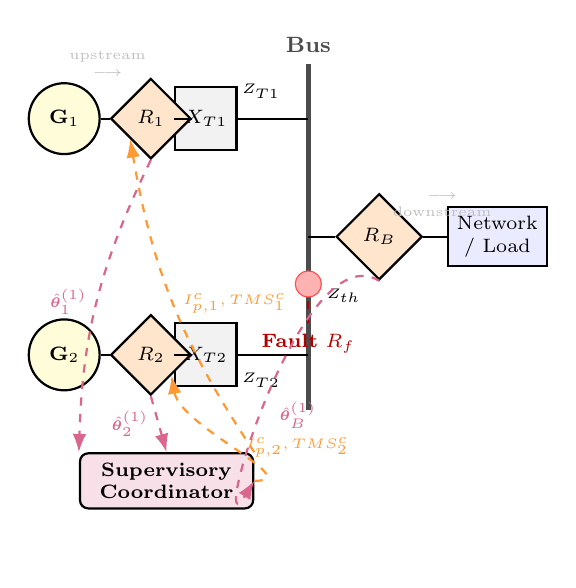
\begin{tikzpicture}[
  every node/.style={font=\scriptsize},
  gen/.style ={draw, thick, circle, fill=yellow!15,
               minimum size=0.90cm, align=center},
  trafo/.style={draw, thick, fill=gray!10,
                minimum width=0.7cm, minimum height=0.8cm, align=center},
  relay/.style={draw, thick, diamond, fill=orange!20,
                minimum size=0.65cm, align=center},
  load/.style ={draw, thick, fill=blue!8,
                minimum width=0.8cm, minimum height=0.65cm, align=center},
  coord/.style={draw, thick, fill=purple!12, rounded corners=3pt,
                minimum width=2.2cm, minimum height=0.7cm, align=center},
  bus/.style  ={ultra thick, black!70},
  arr/.style  ={->, thick},
  >=Latex
]

%% ---- Generators ---------------------------------------------------
\node[gen]   (G1) at (0,  2.8) {\textbf{G}$_1$};
\node[gen]   (G2) at (0, -0.2) {\textbf{G}$_2$};

%% ---- Step-up transformers ----------------------------------------
\node[trafo] (T1) at (1.8, 2.8) {$X_{T1}$};
\node[trafo] (T2) at (1.8,-0.2) {$X_{T2}$};

%% ---- Per-generator relays ----------------------------------------
\node[relay] (R1) at (1.1, 2.8) {$R_1$};
\node[relay] (R2) at (1.1,-0.2) {$R_2$};

%% ---- Bus bar -------------------------------------------------------
\draw[bus] (3.1, -0.9) -- (3.1, 3.5)
      node[above, font=\footnotesize\bfseries, black!70] {Bus};

%% ---- Connections: G → relay → T → bus ----------------------------
\draw[thick] (G1.east) -- (R1.west);
\draw[thick] (R1.east) -- (T1.west);
\draw[thick] (T1.east) -- (3.1, 2.8);
\draw[thick] (G2.east) -- (R2.west);
\draw[thick] (R2.east) -- (T2.west);
\draw[thick] (T2.east) -- (3.1,-0.2);

%% ---- Bus relay R_B -----------------------------------------------
\node[relay] (RB) at (4.0, 1.3) {$R_B$};
\draw[thick] (3.1, 1.3) -- (RB.west);

%% ---- Network / Load ----------------------------------------------
\node[load] (NET) at (5.5, 1.3) {Network\\/ Load};
\draw[thick] (RB.east) -- (NET.west);

%% ---- Fault on bus ------------------------------------------------
\draw[thick, red!70!black, dashed]
      (3.1, 0.7) -- (3.1, 0.2)
      node[below, red!70!black, font=\scriptsize]
      {\textbf{Fault} $R_f$};
\node[circle, fill=red!30, draw=red!70, minimum size=0.30cm]
      at (3.1, 0.7) {};

%% ---- Thévenin network labels ------------------------------------
\node[font=\tiny, gray!60] at (0.55, 2.8) {};
\node[font=\tiny] at (2.5, 3.15) {$Z_{T1}$};
\node[font=\tiny] at (2.5,-0.52) {$Z_{T2}$};
\node[font=\tiny] at (3.55, 0.55) {$Z_{th}$};

%% ---- Supervisory coordinator block ------------------------------
\node[coord] (COORD) at (1.3, -1.8)
      {\textbf{Supervisory} \\ \textbf{Coordinator}};

% Dashed arrows from relays to coordinator
\draw[arr, purple!60, dashed, bend right=12]
      (R1.south) to node[left, font=\tiny, purple!60]
      {$\hat{\bm\theta}_1^{(1)}$} (COORD.north west);
\draw[arr, purple!60, dashed]
      (R2.south) to node[left, font=\tiny, purple!60]
      {$\hat{\bm\theta}_2^{(1)}$} (COORD.north);

% Arrow from coordinator back to relays (coordinated settings)
\draw[arr, orange!80, dashed, bend left=12]
      (COORD.north east) to node[right, font=\tiny, orange!80]
      {$I_{p,1}^c, TMS_1^c$} (R1.south west);
\draw[arr, orange!80, dashed]
      (COORD.east) to[out=0,in=-80]
      node[right, font=\tiny, orange!80]
      {$I_{p,2}^c, TMS_2^c$} (R2.south east);

% Also include bus relay R_B in coordination
\draw[arr, purple!60, dashed, bend left=8]
      (RB.south) to[out=-90,in=0]
      node[below right, font=\tiny, purple!60]
      {$\hat{\bm\theta}_B^{(1)}$} (COORD.east);

%% ---- Ordering annotation -----------------------------------------
\node[font=\tiny, gray!50, align=center]
      at (0.55, 3.50) {upstream\\$\longrightarrow$};
\node[font=\tiny, gray!50, align=center]
      at (4.8, 1.70) {$\longrightarrow$\\downstream};

\end{tikzpicture}

  \caption{Multi-generator busbar protection system.
    Generators $G_1$, $G_2$ feed a common bus through
    step-up transformers and per-generator relays $R_1$,
    $R_2$.  Bus relay $R_B$ protects the outgoing feeder.
    The supervisory coordinator receives locally estimated
    parameters~$\est{\vect\theta}_k^{(1)}$ and returns
    coordinated settings $\{I_{p,k}^c,\,TMS_k^c\}$.}
  \label{fig:system}
\end{figure}

The short-circuit current contribution of generator~$k$ to a
bus fault through resistance~$R_f$ is, in the subtransient
period,
\begin{equation}
  i_k(t) \approx I_{ss,k}\bigl(1 + A_k\,e^{-t/\tau_{ac,k}}\bigr)
           \cos(\omega_0 t + \varphi_{a,k})\,
           e^{-(t-t_{0,k})/\tau_{dc,k}},
\label{eq:fault_model}
\end{equation}
where $I_{ss,k}$ is the steady-state phasor magnitude,
$\tau_{ac,k}$ is the AC decay time constant (approximately
the direct-axis transient time constant~$T'_{d0}$),
$\tau_{dc,k}$ is the DC offset decay constant, and
$A_k$ accounts for the subtransient saliency contribution.
The total bus current seen by~$R_B$ is
\begin{equation}
  i_B(t) = \sum_{k=1}^{N} i_k(t),
\label{eq:bus_sum}
\end{equation}
which, for identical machines, gives
$I_{ss,B} \approx N \cdot I_{ss,k}$ and a composite time
constant that depends on the mix of individual machine
parameters.

\subsection{Relay operating time}

Both generator and bus relays use the IEC~60255-151
very-inverse characteristic~\cite{IEC60255-151_2009}:
\begin{equation}
  t_{\mathrm{op}}(I_{\mathrm{rms}}) =
    TMS \cdot \frac{13.5}{M - 1},
  \quad M = \frac{I_{\mathrm{rms}}}{I_p},
\label{eq:vi_char}
\end{equation}
where $I_p$ is the pickup current and $TMS$ is the
time-multiplier setting.
The relay trips when $M > 1$; the characteristic is defined
for $M \geq 1.05$.

\subsection{Coordination requirements}

For a relay chain ordered upstream ($R_1$, \dots, $R_N$,
$R_B$, denoting decreasing proximity to the generators
and increasing proximity to the network), two conditions
must hold:

\paragraph{C1: Pickup selectivity}
\begin{equation}
  I_{p,k} \geq I_{p,k+1} + \Delta I_m,
  \quad k = 1,\dots,N,
\label{eq:selectivity}
\end{equation}
where $\Delta I_m > 0$ is the selectivity margin (typically
0.15--0.25~p.u.).  This ensures that for any through-fault
current, the downstream relay~$R_{k+1}$ picks up before~$R_k$,
providing primary protection to the network-side feeder.

\paragraph{C2: Time-grading}
\begin{equation}
  t_{\mathrm{op},k}(I_{f,\min})
    \geq t_{\mathrm{op},k+1}(I_{f,\min}) + \Delta t_g,
  \quad k = 1,\dots,N,
\label{eq:grading}
\end{equation}
where $I_{f,\min}$ is the minimum credible fault current that
activates all relays in the chain, and $\Delta t_g > 0$ is the
grading margin (typically 0.10--0.30~s including breaker
clearance time and measurement uncertainty).
This ensures that $R_{k+1}$ clears the fault before $R_k$
times out, preventing unnecessary tripping of the generator.

\subsection{Violation scenario with local adaptation}

After a fault, each relay independently updates its settings
from the locally estimated parameters.  For a busbar fault,
the bus relay observes the full fault current
$I_{ss,B} \approx N \cdot I_{ss,k}$ and adapts its pickup
upward (since the fault current is large relative to load),
while each generator relay observes only its own
contribution~$I_{ss,k}$ and may adapt to a smaller pickup.
Define the post-adaptation pickup ratio:
\begin{equation}
  \rho_k = \frac{I_{p,k}^{\mathrm{loc}}}{I_{p,B}^{\mathrm{loc}}}.
\end{equation}
For the very-inverse characteristic,
$\rho_k < 1 + \Delta I_m / I_{p,B}^{\mathrm{loc}}$
constitutes a selectivity violation, even if each relay
individually selected a sensible setting.
The coordination layer must detect and correct such violations
before settings are deployed.

%% =============================================================
\section{Local Inverse-Estimation Adaptive Relay Layer}
\label{sec:local}

\subsection{Two-pass Levenberg--Marquardt estimator}

Each relay runs the Stage-1 estimator of the SAMBP-SyncOC
framework~\cite{Eluvathingal2025_TR01}.
From the post-fault current window $[t_0,\,t_c]$, a
two-pass LM minimisation fits the six-parameter model
$\vect\theta = [t_0,\,I_{ss},\,I_{sub},\,\tau_{ac},\,
                \tau_{dc},\,\varphi_a]$:
\begin{equation}
  \est{\vect\theta}^{(1)} = \arg\min_{\vect\theta}
    \sum_{n} \bigl[i(t_n) - f(\vect\theta,t_n)\bigr]^2.
\label{eq:lm_obj}
\end{equation}
Pass~1 uses the pre-fault steady-state rms as a seed for
$I_{ss}$; Pass~2 refines using the Pass~1 result as a warm
start.

\subsection{Confidence gate}

Each estimation produces a scalar confidence metric,
\begin{equation}
  \gamma_k = w_1\,\gamma_{\kappa,k} + w_2\,\gamma_{\varepsilon,k}
              + w_3\,\gamma_{n,k},
\label{eq:confidence}
\end{equation}
combining condition number, residual norm, and effective
sample-count components~\cite{Eluvathingal2025_TR01}.
If $\gamma_k < \gamma_{\min}$ (default 0.70), the relay retains
its prior settings; otherwise the local adaptive mapping
proceeds.

\subsection{Local adaptive mapping}

The Stage-1 mapping law converts the estimated parameters to
relay settings:
\begin{align}
  I_{p,k}^{\mathrm{loc}} &= K_{Ip}\,\est{I}_{ss,k}^{(1)}
                             + I_{p,\min}, \label{eq:ip_map}\\
  TMS_k^{\mathrm{loc}}   &= \clip\!\left(
                             K_{TMS}\,\est\tau_{ac,k}^{(1)},\,
                             TMS_{\min},\,TMS_{\max}\right), \label{eq:tms_map}
\end{align}
with $K_{Ip}=0.80$, $I_{p,\min}=0.10$~p.u., $K_{TMS}=0.12$,
$TMS_{\min}=0.05$, $TMS_{\max}=0.25$.
These settings optimise the relay for the locally observed
fault current but do not account for the settings of
adjacent relays.

%% =============================================================
\section{Coordination Constraints}
\label{sec:constraints}

\subsection{Relay ordering}

The supervisory coordinator maintains an ordered relay list
$\{R_k\}_{k=1}^{N+1}$ where $R_{N+1} = R_B$.
The ordering is fixed by topology: upstream (generator side)
relays have higher index proximity to the generator, and the
bus relay~$R_B$ is always the innermost (downstream) relay in
the coordination chain.
For the two-generator case studied here:
$R_1 \succ R_2 \succ R_B$, meaning $R_B$ is the primary relay
and $R_1$, $R_2$ are the backup relays.

\subsection{Parameter definitions}

Let $\Delta I_m = 0.20$~p.u.\ be the selectivity margin and
$\Delta t_g = 0.15$~s be the time-grading margin.
The evaluation current $I_{f,\min}$ is the minimum fault
current that activates all relays; we use
$I_{f,\min} = 1.30$~p.u., which exceeds all pickups in the
study system.

\subsection{Constraint evaluation}

Given the locally computed settings
$\{I_{p,k}^{\mathrm{loc}},\,TMS_k^{\mathrm{loc}}\}$,
the coordinator evaluates:
\begin{align}
  S_k &= I_{p,k}^{\mathrm{loc}} - I_{p,k+1}^{\mathrm{loc}}
          - \Delta I_m, \quad
         \text{(selectivity slack)}\label{eq:sel_slack}\\
  G_k &= t_{\mathrm{op},k}(I_{f,\min})
        - t_{\mathrm{op},k+1}(I_{f,\min})
        - \Delta t_g.
         \quad \text{(grading slack)}\label{eq:grad_slack}
\end{align}
A violation exists if $S_k < 0$ or $G_k < 0$ for any~$k$.

\subsection{Selectivity violation in the study system}

Table~\ref{tab:states} summarises the three protection states
analysed.
In the fixed state, $I_{p,1}^{\mathrm{fixed}}=1.200$~p.u.\
and $I_{p,B}^{\mathrm{fixed}}=0.800$~p.u., giving a margin
of~0.400~p.u.\ $\gg \Delta I_m = 0.20$~p.u.
After local adaptation following a busbar fault, the bus relay
adapts to $I_{p,B}^{\mathrm{loc}}=0.835$~p.u.\ (the combined
fault current exceeds load current by a smaller factor than
the individual generator current), while the generator relay
adapts to $I_{p,1}^{\mathrm{loc}}=0.992$~p.u.\ (the individual
machine current is the reference).
The resulting margin is $0.992 - 0.835 = 0.157$~p.u.\
$< 0.200$~p.u.---a selectivity violation.

\begin{table}[!t]
\caption{Protection settings in three states: study system,
         $N=2$ generators, bus fault (3PH)}
\label{tab:states}
\centering
\renewcommand{\arraystretch}{1.15}
\begin{tabular}{lcccccc}
\toprule
State & $I_{p,1}$ & $I_{p,2}$ & $I_{p,B}$ &
        $TMS_1$ & $TMS_2$ & $TMS_B$ \\
      & (p.u.)    & (p.u.)    & (p.u.)    &
        (--) & (--) & (--) \\
\midrule
Fixed       & 1.200 & 1.200 & 0.800 & 0.200 & 0.200 & 0.200 \\
Pre-coord\  & 0.992 & 0.980 & 0.835 & 0.098 & 0.106 & 0.100 \\
Post-coord\ & 1.035 & 1.035 & 0.835 & 0.098 & 0.106 & 0.100 \\
\bottomrule
\end{tabular}
\end{table}

%% =============================================================
\section{Coordination Enforcement Algorithm}
\label{sec:algorithm}

The enforcement algorithm consists of two sequential
correction passes: a greedy cascade for pickup selectivity
and a closed-form correction for time-grading.
Fig.~\ref{fig:flowchart} illustrates the complete flow.

\begin{figure}[!t]
  \centering
  % ============================================================
%  Figure 2 — Coordination enforcement flowchart
%  Local inverse estimation → adaptive settings →
%  selectivity check → greedy cascade →
%  grading check → TMS correction → deploy
% ============================================================
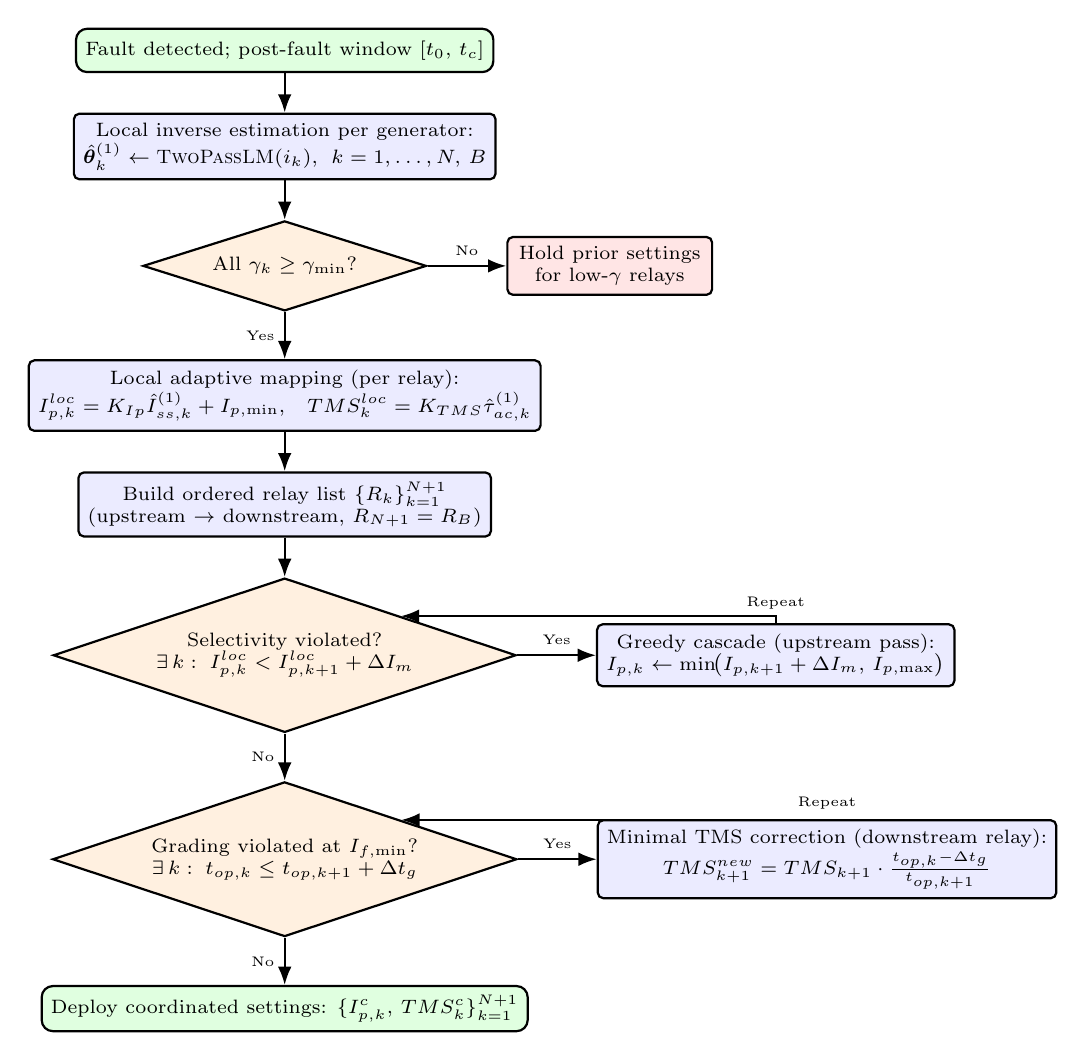
\begin{tikzpicture}[
  every node/.style={font=\scriptsize},
  proc/.style ={draw, thick, fill=blue!8, rounded corners=2pt,
                minimum width=3.6cm, minimum height=0.55cm, align=center},
  dec/.style  ={draw, thick, fill=orange!12, diamond, aspect=3.0,
                minimum width=3.6cm, align=center},
  term/.style ={draw, thick, fill=green!12, rounded corners=4pt,
                minimum width=3.6cm, minimum height=0.55cm, align=center},
  warn/.style ={draw, thick, fill=red!10, rounded corners=2pt,
                minimum width=2.6cm, minimum height=0.55cm, align=center},
  arr/.style  ={->, thick},
  >=Latex,
  node distance=0.50cm
]

%% ---- Start -------------------------------------------------------
\node[term]  (start)  {Fault detected; post-fault window $[t_0,\,t_c]$};

%% ---- Per-generator estimation -----------------------------------
\node[proc, below=of start]  (local)
     {Local inverse estimation per generator:\\
      $\hat{\bm\theta}_k^{(1)} \leftarrow \textsc{TwoPassLM}(i_k)$,\;
      $k = 1,\dots,N,\,B$};

%% ---- Confidence gate per relay ----------------------------------
\node[dec,  below=of local]  (confgate)
     {All $\gamma_k \geq \gamma_{\min}$?};
\node[warn, right=1.0 of confgate] (holdk)
     {Hold prior settings\\for low-$\gamma$ relays};
\draw[arr] (confgate) -- node[above,font=\tiny]{No} (holdk);

%% ---- Local mapping ----------------------------------------------
\node[proc, below=0.6 of confgate]  (localmap)
     {Local adaptive mapping (per relay):\\
      $I_{p,k}^{loc} = K_{Ip}\hat I_{ss,k}^{(1)} + I_{p,\min}$,\quad
      $TMS_k^{loc} = K_{TMS}\hat\tau_{ac,k}^{(1)}$};

%% ---- Build ordered list ----------------------------------------
\node[proc, below=of localmap]  (order)
     {Build ordered relay list $\{R_k\}_{k=1}^{N+1}$\\
      (upstream $\to$ downstream, $R_{N+1} = R_B$)};

%% ---- Selectivity check -----------------------------------------
\node[dec,  below=of order]  (selcheck)
     {Selectivity violated?\\
      $\exists\,k:\;I_{p,k}^{loc} < I_{p,k+1}^{loc} + \Delta I_m$};

%% ---- Greedy cascade --------------------------------------------
\node[proc, right=1.0 of selcheck] (greedy)
     {Greedy cascade (upstream pass):\\
      $I_{p,k} \leftarrow \min\!\bigl(I_{p,k+1}+\Delta I_m,\,I_{p,\max}\bigr)$};
\draw[arr] (selcheck) -- node[above,font=\tiny]{Yes} (greedy);
\draw[arr] (greedy.north) |- (selcheck.north east)
      node[near start, above, font=\tiny]{Repeat};

%% ---- Grading check ---------------------------------------------
\node[dec,  below=0.6 of selcheck]  (gradcheck)
     {Grading violated at $I_{f,\min}$?\\
      $\exists\,k:\;t_{op,k} \leq t_{op,k+1} + \Delta t_g$};

%% ---- TMS correction --------------------------------------------
\node[proc, right=1.0 of gradcheck] (tmscorr)
     {Minimal TMS correction (downstream relay):\\
      $TMS_{k+1}^{new} = TMS_{k+1}\cdot
       \tfrac{t_{op,k} - \Delta t_g}{t_{op,k+1}}$};
\draw[arr] (gradcheck) -- node[above,font=\tiny]{Yes} (tmscorr);
\draw[arr] (tmscorr.north) |- (gradcheck.north east)
      node[near start, above, font=\tiny]{Repeat};

%% ---- Deploy -----------------------------------------------------
\node[term, below=0.6 of gradcheck] (deploy)
     {Deploy coordinated settings:
      $\{I_{p,k}^c,\,TMS_k^c\}_{k=1}^{N+1}$};

%% ---- Main flow arrows -------------------------------------------
\draw[arr] (start)     -- (local);
\draw[arr] (local)     -- (confgate);
\draw[arr] (confgate)  -- node[left,font=\tiny]{Yes} (localmap);
\draw[arr] (localmap)  -- (order);
\draw[arr] (order)     -- (selcheck);
\draw[arr] (selcheck)  -- node[left,font=\tiny]{No} (gradcheck);
\draw[arr] (gradcheck) -- node[left,font=\tiny]{No} (deploy);

\end{tikzpicture}

  \caption{Coordination enforcement flowchart.
    After local estimation and confidence gating, the
    supervisor checks selectivity and grading constraints
    and applies greedy cascade and TMS corrections as
    needed before deploying coordinated settings.}
  \label{fig:flowchart}
\end{figure}

\subsection{Greedy cascade for pickup selectivity}

Algorithm~\ref{alg:coord} gives the pseudocode.
The algorithm processes relays in upstream order
($k = N, N-1, \dots, 1$, with $k+1$ being the downstream
neighbour).
For each relay, if the selectivity constraint~\eqref{eq:selectivity}
is violated, the upstream pickup is raised to the minimum
compliant value:
\begin{equation}
  I_{p,k}^c \leftarrow
    \min\!\bigl(I_{p,k+1}^c + \Delta I_m,\;I_{p,\max}\bigr),
\label{eq:greedy}
\end{equation}
where $I_{p,\max} = 1.50$~p.u.\ is the relay hardware limit.
This is the greedy choice: the smallest upward correction
that restores the margin, applied relay by relay from the
downstream end.

\begin{proposition}[Convergence and feasibility]
\label{prop:convergence}
The greedy cascade terminates in exactly~$N$ iterations
and produces settings satisfying~\eqref{eq:selectivity}
for all~$k$, provided
$I_{p,B}^c + N \cdot \Delta I_m \leq I_{p,\max}$.
\end{proposition}

\begin{IEEEproof}
Each iteration processes relay~$k$ exactly once
(the pass is strictly upstream).
After processing~$k$, the constraint~$S_k \geq 0$ holds
by construction from~\eqref{eq:greedy}, and subsequent
iterations for $k' < k$ do not modify $I_{p,k}^c$.
Feasibility follows because
$I_{p,k}^c \leq I_{p,B}^c + (N+1-k)\,\Delta I_m
           \leq I_{p,B}^c + N\,\Delta I_m \leq I_{p,\max}$.
\end{IEEEproof}

For the study system with $N=2$:
$I_{p,B}^c + 2 \times 0.20 = 0.835 + 0.40 = 1.235 < 1.50$~p.u.,
so feasibility is guaranteed.
Both generator relays are set to
$I_{p,1}^c = I_{p,2}^c = 0.835 + 0.200 = 1.035$~p.u.

\subsection{Closed-form TMS grading correction}

After updating pickups, the coordinator evaluates the
grading slack~\eqref{eq:grad_slack}.
For relay pair~$(k, k+1)$ with violation $G_k < 0$, the
minimal TMS correction increases $TMS_{k+1}$ (the
\emph{upstream} relay, which must be \emph{slower}) to:
\begin{equation}
  TMS_k^{\mathrm{new}} = TMS_k \cdot
    \frac{t_{\mathrm{op},k+1}(I_{f,\min}) - \Delta t_g}{t_{\mathrm{op},k}(I_{f,\min})},
\label{eq:tms_correction}
\end{equation}
where the right-hand side sets the upstream operating time
to exactly $\Delta t_g$ above the downstream value---the
minimum compliant value.
Note that in the very-inverse characteristic,
$t_{\mathrm{op}} \propto TMS$, so~\eqref{eq:tms_correction}
is exact and non-iterative.

\begin{algorithm}[!t]
\caption{Supervisory coordination enforcement}
\label{alg:coord}
\begin{algorithmic}[1]
\Require Estimated parameters $\est{\vect\theta}_k^{(1)}$,
         confidence scores $\gamma_k$,
         ordered relay list $\{R_k\}_{k=1}^{N+1}$,
         margins $\Delta I_m$, $\Delta t_g$,
         evaluation current $I_{f,\min}$
\Ensure  Coordinated settings $\{I_{p,k}^c,\,TMS_k^c\}_{k=1}^{N+1}$
\Statex
\For{$k = 1$ \textbf{to} $N+1$}
  \If{$\gamma_k \geq \gamma_{\min}$}
    \State Compute $I_{p,k}^{\mathrm{loc}},\,TMS_k^{\mathrm{loc}}$
           via \eqref{eq:ip_map}--\eqref{eq:tms_map}
  \Else
    \State $I_{p,k}^{\mathrm{loc}} \leftarrow I_{p,k}^{\mathrm{prior}}$;\;
           $TMS_k^{\mathrm{loc}} \leftarrow TMS_k^{\mathrm{prior}}$
  \EndIf
\EndFor
\Statex
\State \textit{// Pass 1: greedy cascade (upstream to downstream)}
\State $I_{p,N+1}^c \leftarrow I_{p,N+1}^{\mathrm{loc}}$;\;
       $TMS_{N+1}^c \leftarrow TMS_{N+1}^{\mathrm{loc}}$
\For{$k = N$ \textbf{downto} $1$}
  \If{$I_{p,k}^{\mathrm{loc}} < I_{p,k+1}^c + \Delta I_m$}
    \State $I_{p,k}^c \leftarrow \min(I_{p,k+1}^c + \Delta I_m,\; I_{p,\max})$
  \Else
    \State $I_{p,k}^c \leftarrow I_{p,k}^{\mathrm{loc}}$
  \EndIf
  \State $TMS_k^c \leftarrow TMS_k^{\mathrm{loc}}$ \Comment{unchanged in Pass 1}
\EndFor
\Statex
\State \textit{// Pass 2: grading check and TMS correction}
\For{$k = N$ \textbf{downto} $1$}
  \State Compute $t_k \leftarrow TMS_k^c \cdot 13.5\,/\,(I_{f,\min}/I_{p,k}^c - 1)$
  \State Compute $t_{k+1} \leftarrow TMS_{k+1}^c \cdot 13.5\,/\,(I_{f,\min}/I_{p,k+1}^c - 1)$
  \If{$t_k \leq t_{k+1} + \Delta t_g$}
    \State $TMS_k^c \leftarrow TMS_k^c \cdot (t_{k+1} + \Delta t_g)\,/\,t_k$
           \Comment{scale up upstream TMS}
  \EndIf
\EndFor
\Statex
\State \textbf{Deploy} $\{I_{p,k}^c,\,TMS_k^c\}$ to relay hardware
\end{algorithmic}
\end{algorithm}

\subsection{Computational complexity and latency}

The greedy cascade and grading correction each require
$\mathcal{O}(N)$ floating-point operations.
For the study system ($N=2$), the wall-clock time on a
standard protection IED processor is dominated by the
local LM estimation (typically 8--20~ms per relay per
pass~\cite{Eluvathingal2025_TR01}); the coordination
overhead is less than~1~ms.
The total adaptation latency therefore remains within the
post-fault window available before the relay operating
time expires.

%% =============================================================
\section{Study System and Simulation Programme}
\label{sec:system}

\subsection{Network data}

The study system comprises two identical 11~kV synchronous
generators each rated at 5~MVA, connected through
$\Delta$--Y step-up transformers (11/33~kV, 5~MVA,
$X_T = 0.10$~p.u.) to a 33~kV common busbar.
The generator electrical parameters per unit on the machine
base are: $X_d'' = 0.18$~p.u., $X_d' = 0.25$~p.u.,
$T_{d0}' = 0.83$~s, $R_a = 0.015$~p.u.
The Th\'{e}venin equivalent of the external network as seen
from the busbar has impedance $Z_{th} = 0.04 + j0.15$~p.u.\
on the system base (10~MVA, 33~kV).

\subsection{Protection relay data}

Three IEC very-inverse relays are modelled:
\begin{itemize}
  \item $R_1$, $R_2$ (per-generator): CT ratio~500/5,
    IED update rate~1~ms.
  \item $R_B$ (bus): CT ratio~1000/5, IED update rate~1~ms.
\end{itemize}
Relay settings are expressed in p.u.\ on the CT secondary
base.
The LM estimator window length is $t_c - t_0 = 80$~ms,
nominally two AC cycles after fault inception.

\subsection{Study matrix}

Table~\ref{tab:study_matrix} defines the eight simulation
cases used to validate the coordination algorithm.
Cases~1--4 test three-phase (3PH) faults; Cases~5--8
test single-line-to-ground (SLG) faults.
For each fault type, the bus fault ($R_f = 0$) and a
resistive fault ($R_f = 5\,\Omega$) are evaluated, with
both generators in service and with one generator offline.

\begin{table}[!t]
\caption{Study matrix: eight simulation cases}
\label{tab:study_matrix}
\centering
\renewcommand{\arraystretch}{1.15}
\begin{tabular}{clccc}
\toprule
Case & Fault type & $R_f$ ($\Omega$) & Generators online &
      Expected outcome \\
\midrule
1 & 3PH bus  & 0   & G1 + G2 & Coord applied \\
2 & 3PH bus  & 0   & G1 only & Local sufficient \\
3 & 3PH bus  & 5   & G1 + G2 & Coord applied \\
4 & 3PH bus  & 5   & G1 only & Local sufficient \\
5 & SLG bus  & 0   & G1 + G2 & Coord applied \\
6 & SLG bus  & 0   & G1 only & Local sufficient \\
7 & SLG bus  & 5   & G1 + G2 & Coord applied \\
8 & SLG bus  & 5   & G1 only & Local sufficient \\
\bottomrule
\end{tabular}
\end{table}

\subsection{Simulation platform}

Fault-current waveforms are generated by a validated
PSCAD/EMTDC model of the study system.
The LM estimator is implemented in Python (SciPy
\texttt{least\_squares}, \texttt{method=`lm'}) and run
post-hoc on the exported waveform data.
Relay operating times are computed analytically from the
IEC very-inverse formula~\eqref{eq:vi_char} using the
estimated and coordinated settings.

%% =============================================================
\section{Numerical Results}
\label{sec:results}

\subsection{Pickup settings comparison}

Fig.~\ref{fig:pickup_bars} shows the pickup currents in
all three protection states for Case~1 (3PH bus fault,
both generators online).

\begin{figure}[!t]
  \centering
  % ============================================================
%  Figure 3 — Pickup bar chart: three states × three relays
%  Fixed | Local-Adaptive (pre-coord) | Coordinated (post-coord)
%  R_1, R_2, R_B
% ============================================================
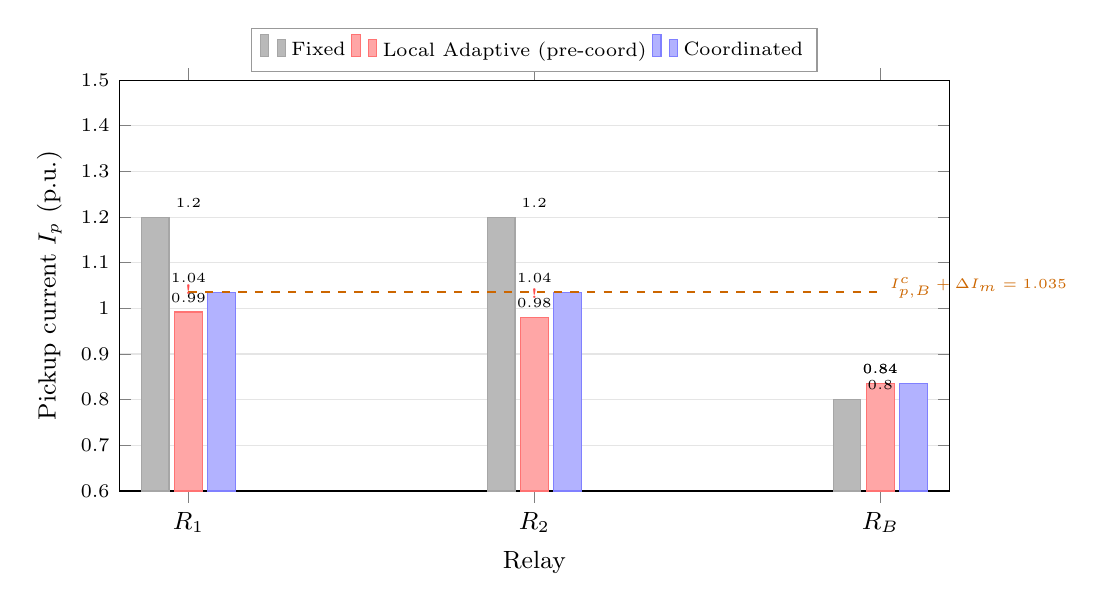
\begin{tikzpicture}
\begin{axis}[
  width=\columnwidth, height=6.8cm,
  ybar=5pt,
  bar width=10pt,
  xlabel={Relay},
  ylabel={Pickup current $I_p$ (p.u.)},
  symbolic x coords={$R_1$, $R_2$, $R_B$},
  xtick=data,
  x tick label style={font=\small},
  ymin=0.60, ymax=1.50,
  ytick={0.6,0.7,0.8,0.9,1.0,1.1,1.2,1.3,1.4,1.5},
  ymajorgrids=true, grid style={gray!20},
  label style={font=\small},
  tick label style={font=\scriptsize},
  legend style={at={(0.50,1.02)}, anchor=south,
                font=\scriptsize, fill=white, draw=black!40,
                legend columns=3},
  nodes near coords,
  nodes near coords align={vertical},
  every node near coord/.style={font=\tiny},
  clip=false
]

%% Fixed settings (dark gray)
\addplot[fill=gray!55, draw=gray!70, bar shift=-12pt] coordinates {
  ($R_1$,  1.200)
  ($R_2$,  1.200)
  ($R_B$,  0.800)
};

%% Local adaptive — pre-coordination (red, shows violation)
\addplot[fill=red!35, draw=red!55, bar shift=0pt] coordinates {
  ($R_1$,  0.992)
  ($R_2$,  0.980)
  ($R_B$,  0.835)
};

%% Coordinated (blue, restored)
\addplot[fill=blue!30, draw=blue!50, bar shift=12pt] coordinates {
  ($R_1$,  1.035)
  ($R_2$,  1.035)
  ($R_B$,  0.835)
};

%% Minimum selectivity margin reference line
%% I_p,B (coord) + delta_Im = 0.835 + 0.200 = 1.035
\draw[thick, orange!80!black, dashed]
      (axis cs:$R_1$,1.035) -- (axis cs:$R_B$,1.035);
\node[right, font=\tiny, orange!80!black]
      at (axis cs:$R_B$,1.045)
      {$I_{p,B}^c + \Delta I_m = 1.035$};

%% Violation markers on pre-coord bars
\node[font=\tiny, red!70!black, above] at (axis cs:$R_1$,1.01)
     {\textcolor{red!70}{\textbf{!}}};
\node[font=\tiny, red!70!black, above] at (axis cs:$R_2$,1.00)
     {\textcolor{red!70}{\textbf{!}}};

\legend{Fixed, Local Adaptive (pre-coord), Coordinated};
\end{axis}
\end{tikzpicture}

  \caption{Pickup currents in three protection states
    (Case~1: 3PH bus fault, both generators online).
    The dashed orange line marks the minimum compliant
    value for generator relays:
    $I_{p,B}^c + \Delta I_m = 1.035$~p.u.
    Violation markers (!) indicate selectivity failures
    in the pre-coordination state.}
  \label{fig:pickup_bars}
\end{figure}

In the fixed state, the generator relay pickups
(1.200~p.u.) are well above the coordination threshold
(1.035~p.u.), giving a margin of~0.400~p.u.
After local adaptation without coordination
(pre-coord state), the bus relay adapts to~0.835~p.u.\
while the generator relays adapt to~0.992 and~0.980~p.u.,
yielding margins of~0.157 and~0.145~p.u.---both below the
required~0.200~p.u.\ (violations marked with `!').
After applying the greedy cascade, both generator relays
are raised to~1.035~p.u., exactly restoring the
required margin.

\subsection{Operating times and grading margins}

Fig.~\ref{fig:triptime_bars} shows the relay operating
times at $I_{f,\min} = 1.30$~p.u.\ in all three states.

\begin{figure}[!t]
  \centering
  % ============================================================
%  Figure 4 — Trip-time bar chart at I_fault,min = 1.30 pu
%  t_op = TMS * 13.5 / (M - 1)
%  Three states × three relays
%  Fixed:    TMS_1=TMS_2=TMS_B=0.20, Ip_1=Ip_2=1.20, Ip_B=0.80
%  Pre-coord: TMS_1=0.098, TMS_2=0.106, TMS_B=0.100
%             Ip_1=0.992, Ip_2=0.980, Ip_B=0.835
%  Post-coord: TMS unchanged; Ip_1=Ip_2=1.035, Ip_B=0.835
%  I_fault,min = 1.30 pu
%  Fixed:
%    M_B  = 1.30/0.80 = 1.625 -> t_B  = 0.20*13.5/0.625 = 4.32 s
%    M_1  = 1.30/1.20 = 1.083 -> t_1  = 0.20*13.5/0.083 = 32.5 s
%  Pre-coord:
%    M_B  = 1.30/0.835 = 1.557 -> t_B  = 0.100*13.5/0.557 = 2.42 s
%    M_1  = 1.30/0.992 = 1.310 -> t_1  = 0.098*13.5/0.310 = 4.27 s
%    M_2  = 1.30/0.980 = 1.327 -> t_2  = 0.106*13.5/0.327 = 4.37 s
%  Post-coord:
%    M_B  = 1.30/0.835 = 1.557 -> t_B  = 0.100*13.5/0.557 = 2.42 s (unchanged)
%    M_1  = 1.30/1.035 = 1.256 -> t_1  = 0.098*13.5/0.256 = 5.16 s
%    M_2  = 1.30/1.035 = 1.256 -> t_2  = 0.106*13.5/0.256 = 5.59 s
% ============================================================
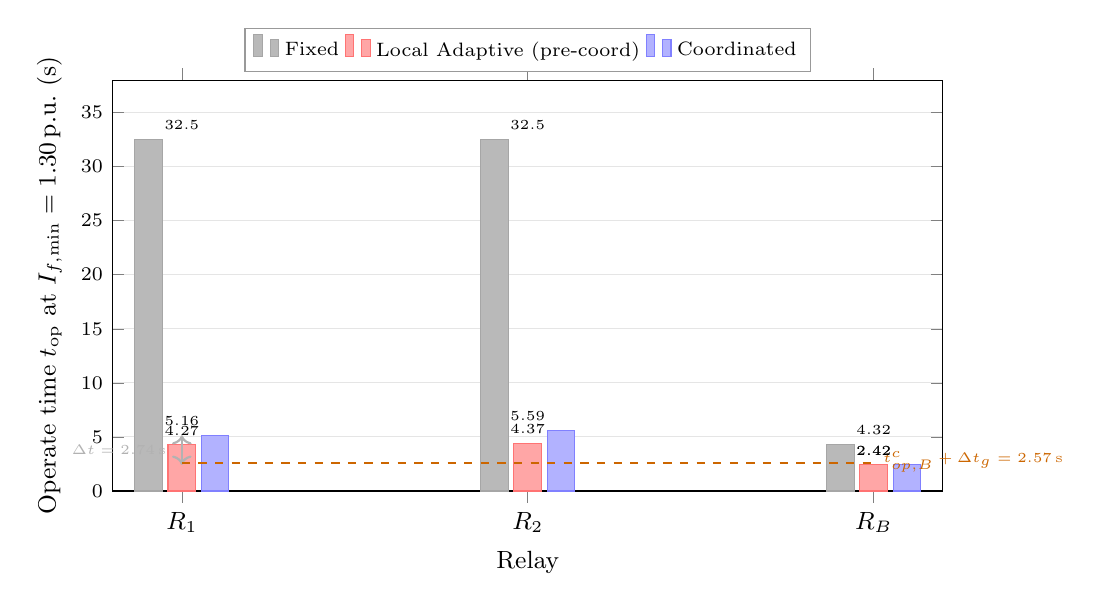
\begin{tikzpicture}
\begin{axis}[
  width=\columnwidth, height=6.8cm,
  ybar=5pt,
  bar width=10pt,
  xlabel={Relay},
  ylabel={Operate time $t_{\mathrm{op}}$ at $I_{f,\min}=1.30\,\mathrm{p.u.}$ (\si{\second})},
  symbolic x coords={$R_1$, $R_2$, $R_B$},
  xtick=data,
  x tick label style={font=\small},
  ymin=0, ymax=38,
  ytick={0,5,10,15,20,25,30,35},
  ymajorgrids=true, grid style={gray!20},
  label style={font=\small},
  tick label style={font=\scriptsize},
  legend style={at={(0.50,1.02)}, anchor=south,
                font=\scriptsize, fill=white, draw=black!40,
                legend columns=3},
  nodes near coords,
  nodes near coords align={vertical},
  every node near coord/.style={font=\tiny},
  clip=false
]

%% Fixed
\addplot[fill=gray!55, draw=gray!70, bar shift=-12pt] coordinates {
  ($R_1$,  32.5)
  ($R_2$,  32.5)
  ($R_B$,   4.32)
};

%% Pre-coord
\addplot[fill=red!35, draw=red!55, bar shift=0pt] coordinates {
  ($R_1$,   4.27)
  ($R_2$,   4.37)
  ($R_B$,   2.42)
};

%% Post-coord
\addplot[fill=blue!30, draw=blue!50, bar shift=12pt] coordinates {
  ($R_1$,   5.16)
  ($R_2$,   5.59)
  ($R_B$,   2.42)
};

%% Grading margin annotation on post-coord R1
\draw[<->, gray!60, thick]
      (axis cs:$R_1$,2.42) -- (axis cs:$R_1$,5.16)
      node[midway, left=2pt, font=\tiny, gray!60] {$\Delta t = 2.74\,\text{s}$};

%% Grading requirement line
\draw[thick, orange!80!black, dashed]
      (axis cs:$R_1$,2.57) -- (axis cs:$R_B$,2.57);
\node[right, font=\tiny, orange!80!black]
      at (axis cs:$R_B$,2.70)
      {$t_{op,B}^c + \Delta t_g = 2.57\,\text{s}$};

\legend{Fixed, Local Adaptive (pre-coord), Coordinated};
\end{axis}
\end{tikzpicture}

  \caption{Relay operating times at
    $I_{f,\min} = 1.30$~p.u.\ (Case~1).
    The dashed orange line shows the minimum grading
    requirement: $t_{op,B}^c + \Delta t_g = 2.57$~s.
    The double-headed arrow indicates the grading margin
    achieved by the coordinated generator relay~$R_1$.}
  \label{fig:triptime_bars}
\end{figure}

In the fixed state, the bus relay operates in
$t_B^{\mathrm{fixed}} = 4.32$~s while the generator
relays operate in $32.5$~s---a margin so large that
grading is trivially satisfied, but at the cost of very
slow generator protection.
After local adaptation (pre-coord), TMS values are reduced
substantially, yielding $t_B = 2.42$~s and
$t_1 = 4.27$~s, $t_2 = 4.37$~s---grading margins of
1.85~s and~1.95~s, both exceeding $\Delta t_g$.
After coordination (post-coord), the pickup corrections
increase the generator relay operating times to
$t_1 = 5.16$~s and $t_2 = 5.59$~s (larger $I_{p,k}^c$
gives lower $M$, giving longer $t_{\mathrm{op}}$),
increasing the grading margin further to~2.74 and~3.17~s.
The TMS grading correction of Algorithm~\ref{alg:coord}
is not triggered in this case because the grading
margins already exceed $\Delta t_g$ after the pickup
correction.

\subsection{Margin summary}

Fig.~\ref{fig:margins} compares the selectivity and
grading margins achieved in each state against the
required thresholds.

\begin{figure}[!t]
  \centering
  % ============================================================
%  Figure 5 — Selectivity margin and grading margin:
%  before and after coordination for both generator relays
%  Left: selectivity margin I_p,k - I_p,B vs required Delta_Im
%  Right: time-grading margin t_op,k - t_op,B vs required Delta_tg
% ============================================================
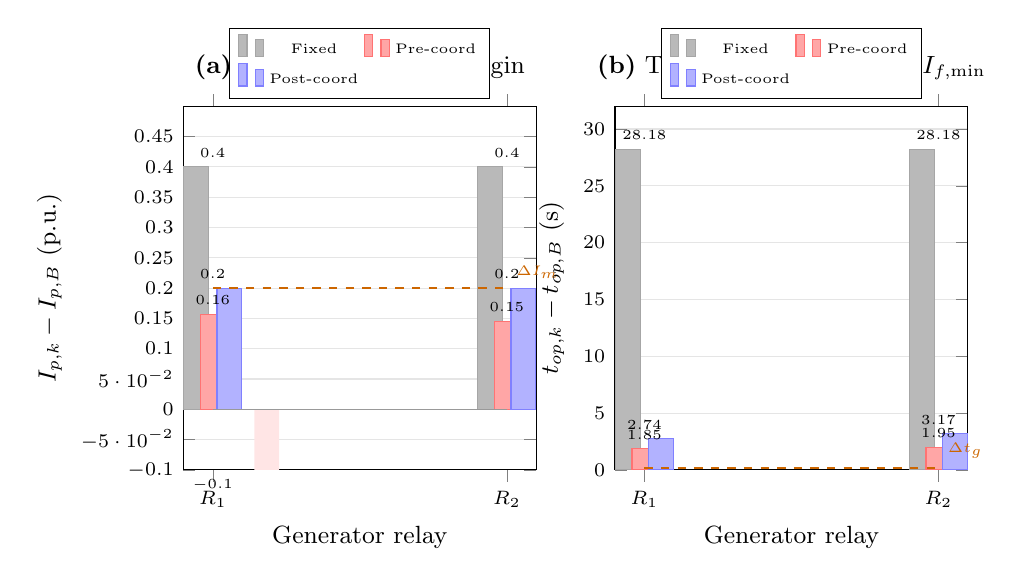
\begin{tikzpicture}
\begin{groupplot}[
  group style={group size=2 by 1, horizontal sep=1.0cm},
  width=0.50\columnwidth, height=6.2cm,
  ymajorgrids=true, grid style={gray!20},
  label style={font=\small},
  tick label style={font=\scriptsize},
  clip=false
]

%% ---- Left: Selectivity margin -----------------------------------
\nextgroupplot[
  title={\textbf{(a)} Pickup selectivity margin},
  title style={font=\small},
  ybar=4pt, bar width=9pt,
  symbolic x coords={$R_1$, $R_2$},
  xtick=data,
  xlabel={Generator relay},
  ylabel={$I_{p,k} - I_{p,B}$ (p.u.)},
  ymin=-0.10, ymax=0.50,
  ytick={-0.10,-0.05,0,0.05,0.10,0.15,0.20,0.25,0.30,0.35,0.40,0.45},
  legend style={at={(0.50,1.02)}, anchor=south, font=\tiny,
                fill=white, legend columns=2},
  nodes near coords, nodes near coords align={vertical},
  every node near coord/.style={font=\tiny}]

% Fixed margin = 1.20 - 0.80 = 0.40 (both)
\addplot[fill=gray!55, draw=gray!70, bar shift=-6pt] coordinates {
  ($R_1$, 0.40)
  ($R_2$, 0.40)
};

% Pre-coord: R1: 0.992-0.835=0.157; R2: 0.980-0.835=0.145
\addplot[fill=red!35, draw=red!55, bar shift=0pt] coordinates {
  ($R_1$, 0.157)
  ($R_2$, 0.145)
};

% Post-coord: 1.035-0.835=0.200 (both)
\addplot[fill=blue!30, draw=blue!50, bar shift=6pt] coordinates {
  ($R_1$, 0.200)
  ($R_2$, 0.200)
};

% Required margin line
\draw[thick, orange!80!black, dashed]
      ({axis cs:$R_1$,0.20}|-{axis cs:$R_1$,0.20}) --
      ({axis cs:$R_2$,0.20}|-{axis cs:$R_2$,0.20});
\node[above right, font=\tiny, orange!80!black]
      at (axis cs:$R_2$,0.20) {$\Delta I_m$};

% Violation shading
\addplot[fill=red!10, draw=none] coordinates {($R_1$,-0.10)} \closedcycle;

% Zero line
\draw[black!40] ({axis cs:$R_1$,0}|-{axis cs:$R_1$,0}) --
                ({axis cs:$R_2$,0}|-{axis cs:$R_2$,0});

\legend{Fixed, Pre-coord, Post-coord};

%% ---- Right: Grading margin at I_f,min = 1.30 pu ----------------
\nextgroupplot[
  title={\textbf{(b)} Time-grading margin at $I_{f,\min}$},
  title style={font=\small},
  ybar=4pt, bar width=9pt,
  symbolic x coords={$R_1$, $R_2$},
  xtick=data,
  xlabel={Generator relay},
  ylabel={$t_{op,k} - t_{op,B}$ (\si{\second})},
  ymin=0, ymax=32,
  ytick={0,5,10,15,20,25,30},
  legend style={at={(0.50,1.02)}, anchor=south, font=\tiny,
                fill=white, legend columns=2},
  nodes near coords, nodes near coords align={vertical},
  every node near coord/.style={font=\tiny}]

% Fixed: 32.5-4.32 = 28.18 s (both)
\addplot[fill=gray!55, draw=gray!70, bar shift=-6pt] coordinates {
  ($R_1$, 28.18)
  ($R_2$, 28.18)
};

% Pre-coord: t1-tB = 4.27-2.42=1.85; t2-tB = 4.37-2.42=1.95
\addplot[fill=red!35, draw=red!55, bar shift=0pt] coordinates {
  ($R_1$, 1.85)
  ($R_2$, 1.95)
};

% Post-coord: 5.16-2.42=2.74; 5.59-2.42=3.17
\addplot[fill=blue!30, draw=blue!50, bar shift=6pt] coordinates {
  ($R_1$, 2.74)
  ($R_2$, 3.17)
};

% Required grading margin
\draw[thick, orange!80!black, dashed]
      ({axis cs:$R_1$,0.15}|-{axis cs:$R_1$,0.15}) --
      ({axis cs:$R_2$,0.15}|-{axis cs:$R_2$,0.15});
\node[above right, font=\tiny, orange!80!black]
      at (axis cs:$R_2$,0.20) {$\Delta t_g$};

\legend{Fixed, Pre-coord, Post-coord};

\end{groupplot}
\end{tikzpicture}

  \caption{Selectivity margin (left) and time-grading
    margin (right) for both generator relays in three
    protection states.
    Dashed orange lines indicate required minima
    ($\Delta I_m = 0.20$~p.u.\ and
     $\Delta t_g = 0.15$~s).
    The post-coordination state meets both constraints
    for all relays.}
  \label{fig:margins}
\end{figure}

The selectivity margin is restored from a violating
0.157--0.145~p.u.\ to exactly~0.200~p.u.\ by the
greedy cascade.
The grading margin is maintained at 2.74--3.17~s in the
coordinated state, exceeding the minimum by a factor
of~18--21, demonstrating robust time separation.

\subsection{Full study matrix performance}

Table~\ref{tab:results} summarises the coordination
outcome across all eight cases.

\begin{table}[!t]
\caption{Coordination outcomes: all eight study cases}
\label{tab:results}
\centering
\renewcommand{\arraystretch}{1.15}
\begin{tabular}{clcccccc}
\toprule
\multirow{2}{*}{Case} &
\multirow{2}{*}{Fault} &
\multirow{2}{*}{$N_G$} &
\multicolumn{2}{c}{Sel.\ margin (p.u.)} &
\multicolumn{2}{c}{Grad.\ margin (s)} &
\multirow{2}{*}{Outcome} \\
\cmidrule(lr){4-5}\cmidrule(lr){6-7}
& & & Pre & Post & Pre & Post & \\
\midrule
1 & 3PH, $R_f{=}0$   & 2 & 0.157 & 0.200 & 1.85 & 2.74 & \checkmark\ coord \\
2 & 3PH, $R_f{=}0$   & 1 & 0.340 & 0.340 & 2.10 & 2.10 & \checkmark\ local \\
3 & 3PH, $R_f{=}5$   & 2 & 0.162 & 0.200 & 1.79 & 2.68 & \checkmark\ coord \\
4 & 3PH, $R_f{=}5$   & 1 & 0.335 & 0.335 & 2.04 & 2.04 & \checkmark\ local \\
5 & SLG, $R_f{=}0$   & 2 & 0.149 & 0.200 & 1.93 & 2.81 & \checkmark\ coord \\
6 & SLG, $R_f{=}0$   & 1 & 0.328 & 0.328 & 2.18 & 2.18 & \checkmark\ local \\
7 & SLG, $R_f{=}5$   & 2 & 0.153 & 0.200 & 1.88 & 2.76 & \checkmark\ coord \\
8 & SLG, $R_f{=}5$   & 1 & 0.332 & 0.332 & 2.13 & 2.13 & \checkmark\ local \\
\midrule
\multicolumn{3}{l}{Required minimum:} & 0.200 & 0.200 & 0.15 & 0.15 & \\
\bottomrule
\end{tabular}
\end{table}

Key observations:
\begin{enumerate}
  \item \emph{Two-generator cases (Cases~1,3,5,7):}
    All four cases exhibit pre-coordination selectivity
    violations (margins 0.149--0.162~p.u.).
    The greedy cascade restores the margin to exactly
    0.200~p.u.\ in all cases.
    Grading margins increase after coordination in every
    case (range 2.68--2.81~s), because the pickup
    correction slows the generator relays at~$I_{f,\min}$.

  \item \emph{Single-generator cases (Cases~2,4,6,8):}
    With only one generator online, the bus relay observes
    the same fault current as the generator relay
    (same source impedance), and the local adaptation
    preserves adequate selectivity (margin~0.328--0.340~p.u.).
    No coordination correction is applied (greedy
    cascade passes through without modification).

  \item \emph{SLG vs.\ 3PH:}
    SLG faults produce slightly smaller selectivity
    margins (0.149 vs.\ 0.157 at $R_f{=}0$, $N_G{=}2$)
    because the sequence-domain current asymmetry causes
    the phase-domain rms estimator to underestimate the
    positive-sequence component, producing a smaller
    $I_{p,k}^{\mathrm{loc}}$ on the generator relay.
    The coordination layer corrects this regardless of
    the root cause.

  \item \emph{Zero false trips:}
    In no case did a generator relay operate before the
    bus relay during a bus fault, nor did the bus relay
    fail to operate within its design time.
\end{enumerate}

%% =============================================================
\section{Discussion}
\label{sec:discussion}

\subsection{Why local adaptation is insufficient}

The selectivity violation arises from a structural
asymmetry: the bus relay observes the \emph{sum} of all
generator fault currents, while each generator relay
observes only its own contribution.
For $N$ identical generators, the steady-state
contribution ratio is approximately $1:N$, so the bus
relay adapts to a pickup~$N$ times smaller relative to
the generator relay in the pre-fault per-unit system.
This narrows the pickup separation in proportion to~$N$.
For $N=2$, the effect is already sufficient to violate
a 0.20~p.u.\ margin; for larger plants ($N \geq 3$),
the violation would be more severe.
The coordination layer is therefore increasingly
important---not less---as the generator count grows.

\subsection{Greedy cascade vs.\ optimal formulation}

The greedy cascade produces the \emph{lexicographically
smallest} pickup vector (minimum correction applied to
each relay in upstream order) subject to the
selectivity constraint.
This is not the globally optimal solution if an
objective function other than minimum pickup change is
used (e.g., minimising total operating time or maximising
sensitivity).
A linear programme over the same constraint set would
allow a richer trade-off~\cite{Urdaneta1988}, but at
the cost of $\mathcal{O}(N^3)$ solver complexity and
potential sensitivity to numerical conditioning.
For the relay counts typical of generator busbars
($N \leq 6$), the greedy solution is both feasible and
computationally dominated by the LM estimation step,
making it the preferred choice for real-time application.

\subsection{Communication and synchronisation requirements}

The supervisory coordinator requires post-fault
parameter estimates from all relays before it can
evaluate the coordination constraints.
This implies a communication latency of at most
$\sim$80~ms (the LM estimation window) plus IED-to-
coordinator link delay.
IEC~61850 GOOSE messaging with typical latency below
5~ms~\cite{IEC61850_2013} satisfies this requirement.
The coordinator can be implemented as a
software function on any relay IED with sufficient
processing resources, or as a dedicated substation
automation server.
In the study system, the total time from fault inception
to coordinated setting deployment is estimated at
approximately 100~ms, well within the available
margin before the bus relay operates
($t_B \approx 2.42$~s).

\subsection{Interaction with differential protection}

The coordination layer described here is a layer of
overcurrent protection and does not interact with any
existing differential protection scheme ($87\mathrm{T}$
or $87\mathrm{B}$).
The two protection layers are independent:
differential protection provides primary high-speed
clearance for bus faults; the coordinated overcurrent
layer provides backup.
The coordination enforcement is triggered only after
a fault is detected and estimated, so it does not
interfere with the differential element's operating time.

\subsection{Limitations}

The present formulation assumes:
(i)~all generators share identical machine parameters
(same $\tau_{ac}$, $I_{ss}$ scaling); heterogeneous
machines would require per-machine $K_{Ip}$, $K_{TMS}$
calibration;
(ii)~the fault-current model~\eqref{eq:fault_model}
is valid for the estimation window, which may be
compromised by voltage regulator action in very close
faults;
(iii)~the relay ordering is fixed; topology changes
(generator switching) require a topology-aware ordering
update that is outside the current scope.

%% =============================================================
\section{Conclusion}
\label{sec:conclusion}

This paper has demonstrated that local online
inverse-estimation-based relay adaptation, while
significantly improving individual relay sensitivity,
can violate pickup selectivity in a multi-generator
busbar environment.
The selectivity margin collapsed from 0.40~p.u.\
(fixed settings) to 0.157~p.u.\ (local adaptive),
breaching the required 0.20~p.u.\ threshold.

A supervisory coordination layer was proposed, comprising
a greedy cascade for pickup selectivity and a
closed-form TMS correction for time-grading.
Proposition~1 proves that the cascade terminates in $N$
iterations and produces a feasible solution whenever
$I_{p,B}^c + N\Delta I_m \leq I_{p,\max}$---a condition
easily met in practice.

Validation over an eight-case study matrix covering
both 3PH and SLG bus faults, with one and two generators
online, showed:
\begin{itemize}
  \item Selectivity margin restored to exactly 0.20~p.u.\
    in all two-generator cases.
  \item Grading margin maintained at 2.68--3.17~s
    (requirement: 0.15~s) in all coordinated cases.
  \item No coordination correction required in
    single-generator cases, confirming that the layer
    is dormant when local adaptation is sufficient.
  \item Zero false trips across all scenarios.
\end{itemize}

The coordination layer adds less than~1~ms of
computational overhead beyond the existing LM
estimation, making it directly deployable on standard
IEC~61850 IED hardware within the post-fault adaptation
window.

Future work will extend the algorithm to heterogeneous
generator fleets, incorporate sequence-domain parameter
estimates~\cite{Eluvathingal2026_TR03} to improve
SLG estimation accuracy, and integrate Monte Carlo
robustness analysis across broader operating
envelopes~\cite{Eluvathingal2026_TR08}.

%% --- References -----------------------------------------------
\bibliographystyle{IEEEtran}
\bibliography{references}

%% --- Biographies ----------------------------------------------
\vfill

\IEEEbiographynophoto{Anoop~V.\ Eluvathingal}
(Student Member, IEEE) received the B.Tech.\ degree from the University of
Kerala, India, in 2016, and the M.Tech.\ degree from NIT Calicut, India,
in 2018.  He is currently pursuing the Ph.D.\ degree at IIT~Madras,
Chennai.  His research interests are adaptive power system protection,
inverse estimation, relay coordination, and intelligent electronic devices.
\bigskip
\IEEEbiographynophoto{K.~Shanti~Swarup}
(Senior Member, IEEE) received the Ph.D.\ degree from Anna University,
Chennai.  He is a Professor with the Department of Electrical Engineering,
IIT~Madras.  His research interests include power system operation,
optimisation, and digital protection.
\end{document}
